\documentclass{article}

\usepackage{graphicx}
\usepackage{tikz}
\usepackage{tikzsymbols}
\usetikzlibrary{calc,patterns,shapes.geometric}
\pagestyle{empty}
\usepackage[margin=0pt]{geometry}
\geometry{papersize={14in,12in}}

\def\centerarc[#1](#2)(#3:#4:#5){\draw[#1] ($(#2)+({#5*cos(#3)},{#5*sin(#3)})$) arc (#3:#4:#5);}

\begin{document}
	\begin{figure}
		\centering
		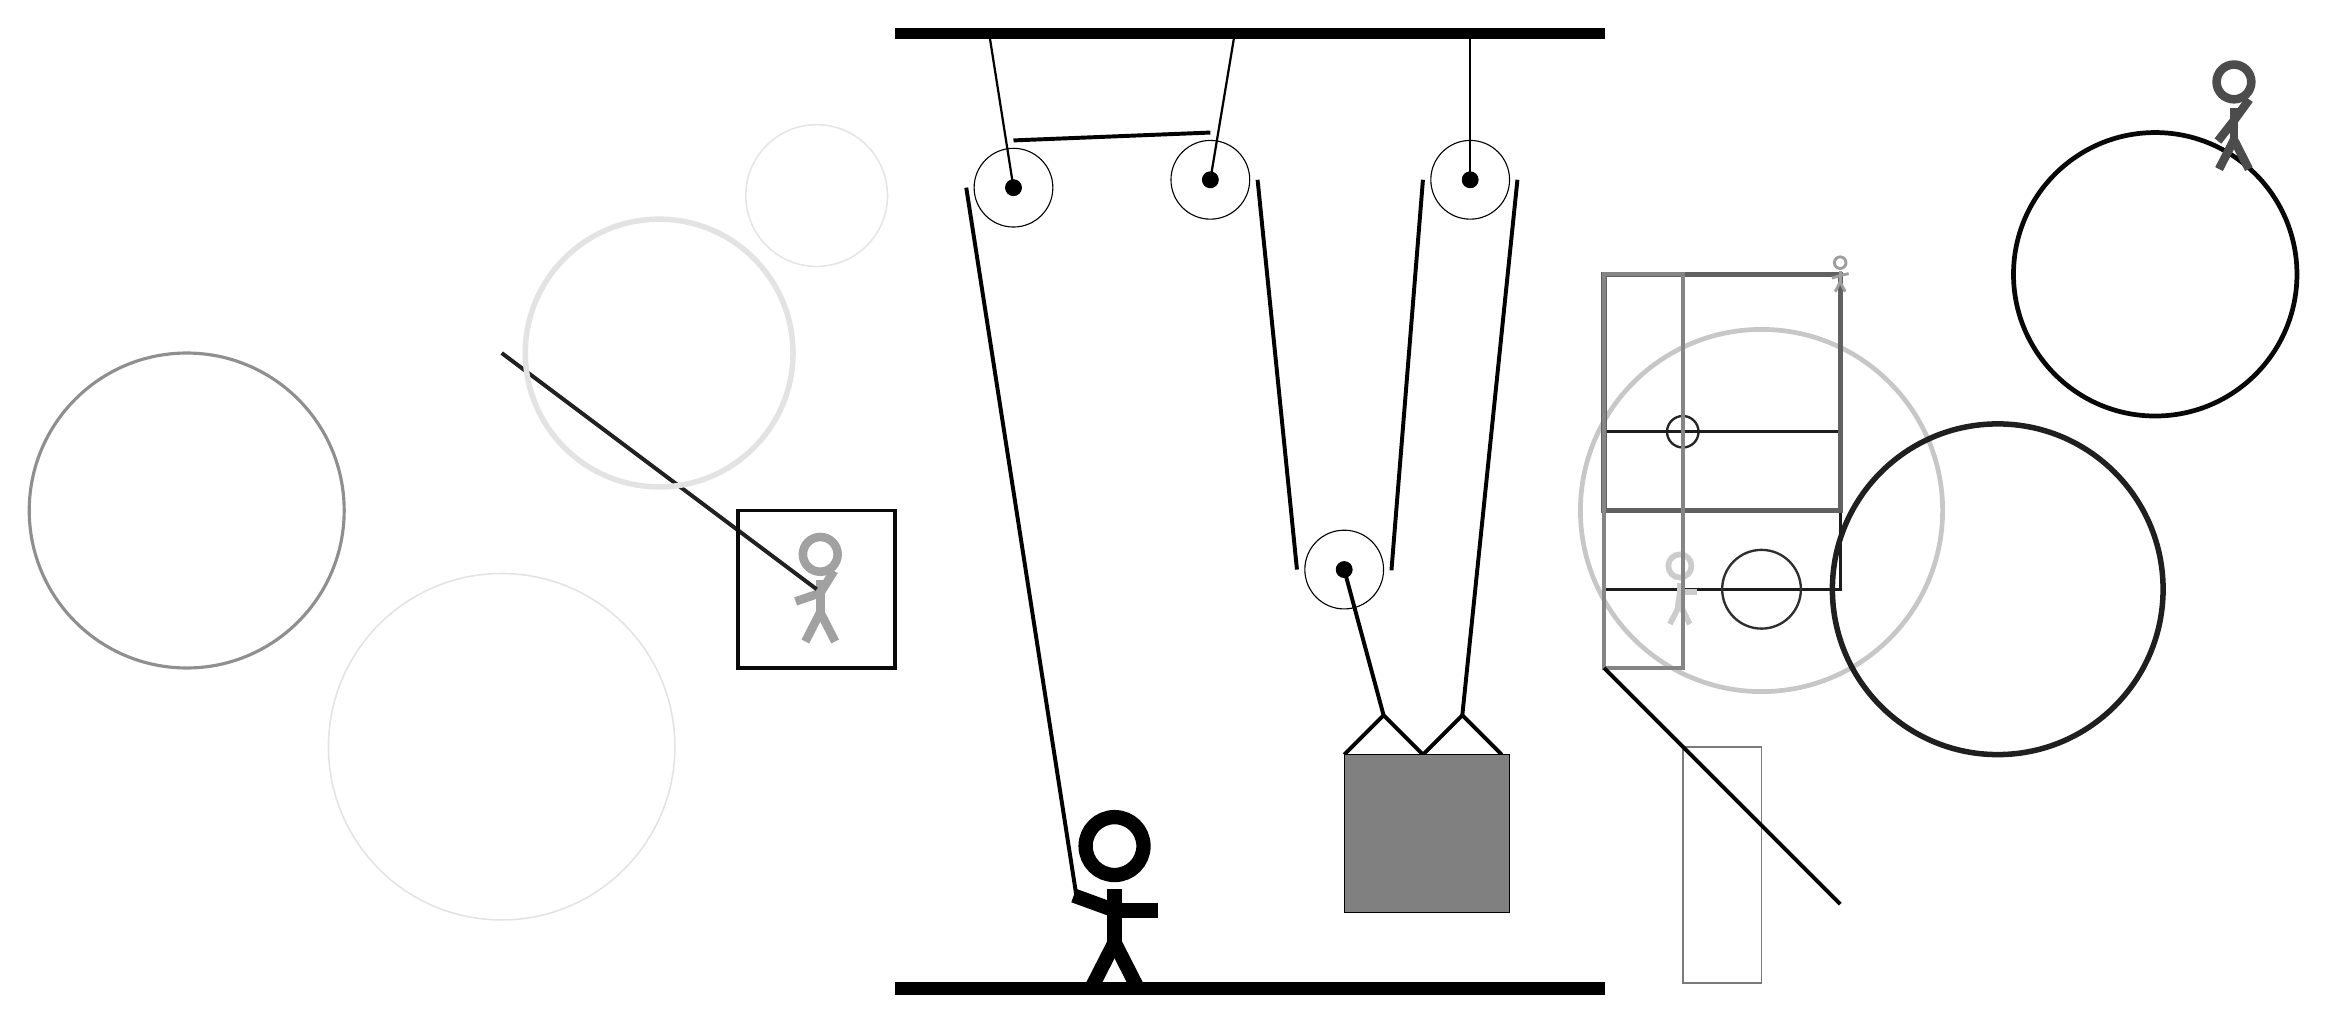
\begin{tikzpicture}
			%%%%% START %%%%%
			
			\draw[fill=black] (-3, 9) rectangle (6, 9.125);
			
			\draw [line width=0.6mm, color=black!97](13, 6) circle (1.8);
			
			\draw [line width=0.3mm, color=black!85](7, 4) circle (0.2);
			\node[line width=0.7mm, color=black!37] at (-4, 2) {\Strichmaxerl[6][19][58]};
			\draw [line width=0.2mm, color=black!10](-4, 7) circle (0.9);
			\draw[line width=0.4mm, color=black!89] (6, 2) rectangle (9, 4);
			\draw[line width=0.5mm, color=black!87](-8, 5) -- (-4, 2);
			
			\draw [line width=0.6mm, color=black!22](8, 3) circle (2.3);
			\draw [line width=0.2mm, color=black!11](-8, 0) circle (2.2);
			\draw[line width=0.7mm, color=black!62] (6, 3) rectangle (9, 6);
			\draw [line width=0.3mm, color=black!82](8, 2) circle (0.5);
			\node[line width=0.4mm, color=black!20] at (7, 2) {\Strichmaxerl[4][82][0]};
			\draw [line width=0.4mm, color=black!44](-12, 3) circle (2.0);
			\node[line width=0.7mm, color=black!70] at (14, 8) {\Strichmaxerl[6][52][54]};
			\draw[line width=0.2mm, color=black!52] (7, -3) rectangle (8, 0);
			\draw [line width=0.7mm, color=black!11](-6, 5) circle (1.7);
			\draw[line width=0.5mm, color=black!96] (-3, 1) rectangle (-5, 3);
			
			\node[line width=0.4mm, color=black!38] at (9, 6) {\Strichmaxerl[2][17][13]};
			
			\draw[line width=0.5mm, color=black!48] (6, 6) rectangle (7, 1);
			\draw [line width=0.7mm, color=black!88](11, 2) circle (2.1);
			
			\draw[line width=0.5mm, color=black!99](6, 1) -- (9, -2);
			
			\draw (1, 7.2) circle (0.5);
			\draw[fill=black] (1, 7.2) circle (0.1);
			\draw[thick] (1, 7.2) -- (1.3, 9);
			
			\draw (4.3, 7.2) circle (0.5);
			\draw[fill=black] (4.3, 7.2) circle (0.1);
			\draw[thick] (4.3, 7.2) -- (4.3, 9);
			
			\draw (2.7, 2.25) circle (0.5);
			\draw[fill=black] (2.7, 2.25) circle (0.1);
			
			\draw[line width=0.5mm]  (2.7, -0.1) -- (3.2, 0.4) -- (3.7, -0.1) -- (4.2, 0.4) -- (4.7, -0.1);
			\draw[fill=black!50] (2.7, -0.1) rectangle (4.8, -2.1);
			
			\draw (-1.5, 7.1) circle (0.5);
			\draw[fill=black] (-1.5, 7.1) circle (0.1);
			\draw[thick] (-1.5, 7.1) -- (-1.8, 9);
			
			\draw[line width=0.5mm](-0.7, -1.9) --  (-2.1, 7.1);
			\centerarc[line width=0.5mm](-1.5, 7.1)(90:180:0.6);
			\draw[line width=0.5mm](-1.5, 7.7) -- (1, 7.8);
			\centerarc[line width=0.5mm](1, 7.2)(0:90:0.6);
			\draw[line width=0.5mm](1.6, 7.2) -- (2.1, 2.25);
			\centerarc[line width=0.5mm](2.7, 2.25)(180:370:0.6);
			\draw[line width=0.5mm] (3.3, 2.24) -- (3.7, 7.2);
			\centerarc[line width=0.5mm](4.3, 7.2)(0:180:0.6);
			\draw[line width=0.5mm](4.2, 0.4) -- (4.9, 7.2);
			\draw[line width=0.5mm] (3.2, 0.4) -- (2.7, 2.25);
			
			\node at (-0.2, -2) {\Strichmaxerl[10][-20][0]};
			
			\draw[fill=black] (-3, -3) rectangle (6, -3.15);
			
			%%%%% END %%%%%
		\end{tikzpicture}
	\end{figure}	
\end{document}